\chapter{Data} \label{chap:data}
Dataset~\cite{dataset} for the project is X-ray images collected at Guangzhou Women and Children’s Medical Center, from pediatric patients aged between one to five.
All X-ray images are in JPEG format and organized into a folder-based structure.
Main sub-structures in the dataset are train, validation and the test folders.
All main folders are also broken into sub-folders that named \emph{Normal} and \emph{Pneumonia} to indicate the classification of the images they contain.
All X-rays have classified by expert physicians and check individually, damaged or un-readable X-rays discarded.
Below are the illustrative examples from both classes of the X-ray.

\begin{figure}[H]%
    \centering
    \subfloat[X-ray without Pnuemonia]{{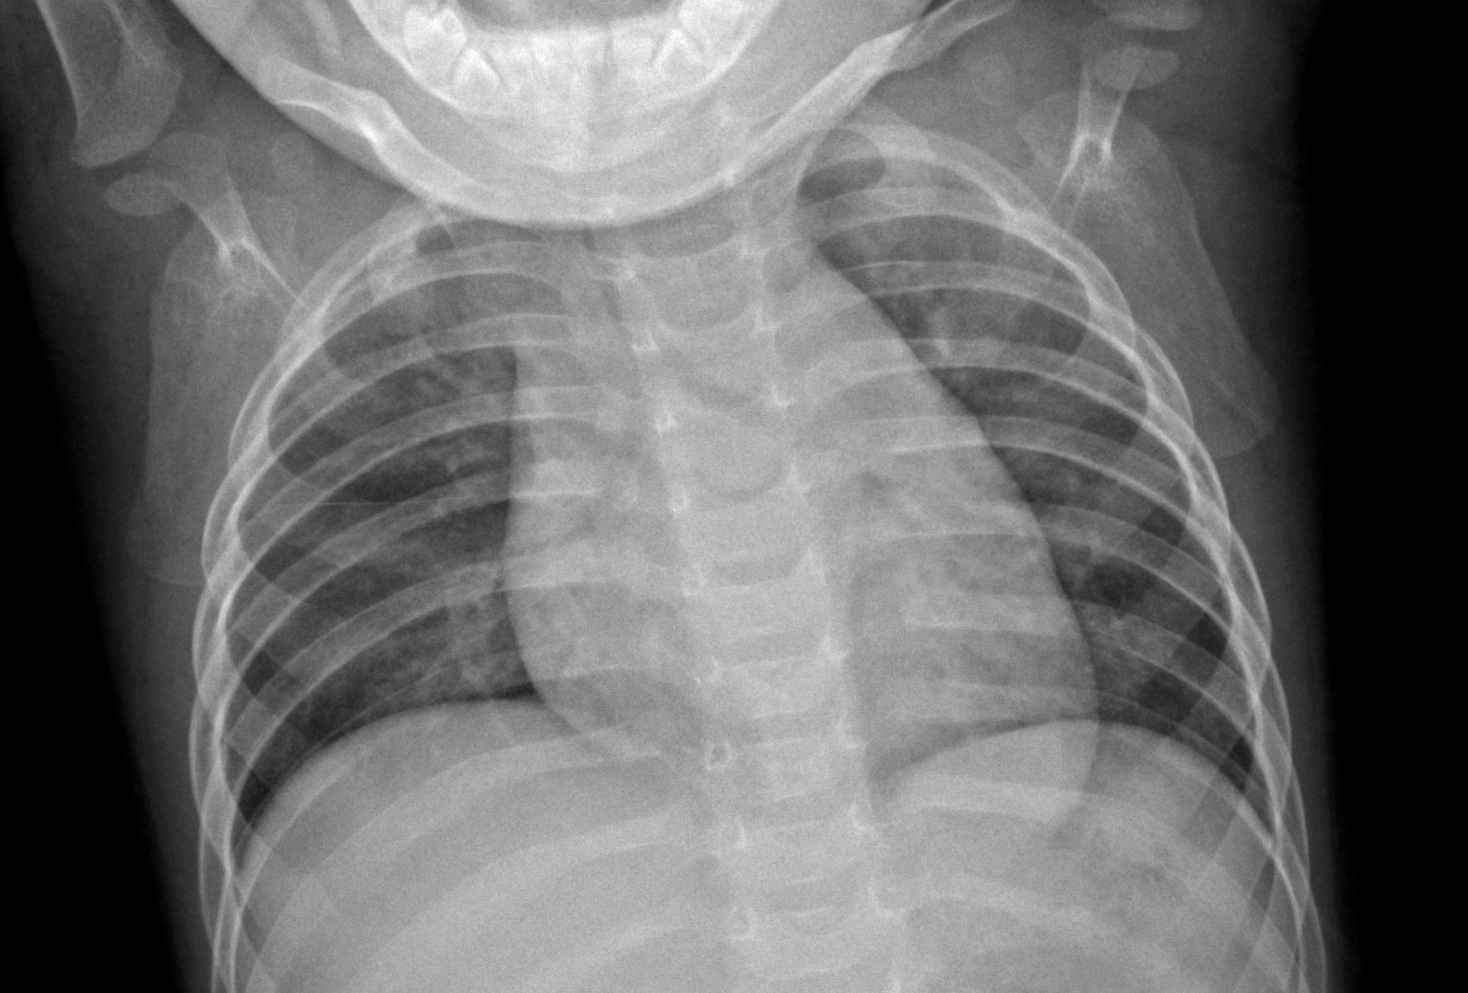
\includegraphics[width=.4\textwidth]{img/chest_xray_train_NORMAL_IM-0133-0001.jpeg} }}%
    \qquad
    \subfloat[X-ray with Pnuemonia]{{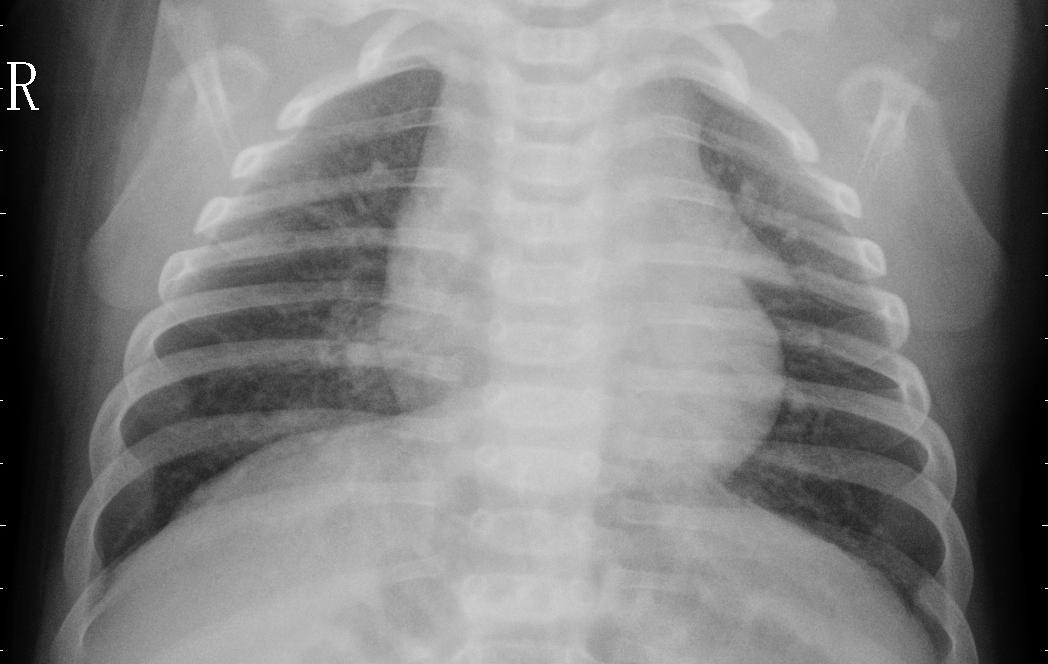
\includegraphics[width=.4\textwidth]{img/chest_xray_train_PNEUMONIA_person1007_virus_1690.jpeg} }}%
    \caption{Two sample X-ray Chest images with and without pneumonia.}%
    \label{fig:sample}%
\end{figure}

For a more detailed understanding of the data, I have checked the content of each train, validation and test datasets. 
There is a significant imbalance in between Pneumonia and Normal classes for train and the test datasets.
A detailed breakdown of each dataset is given in table \ref{table:dataset}.


\begin{table}[H]
    \centering
    \begin{tabular}{||c c c c||} 
    \hline
    Dataset Name & No of images & Pneumonia & Normal \\ [0.5ex] 
    \hline\hline
    Train & 5216 & 3875 & 1341 \\ 
    \hline
    Validation & 16 & 8 & 8 \\
    \hline
    Test & 624 & 390 & 234 \\ [1ex] 
    \hline
    \end{tabular}
    \caption{Breakdown of images for each classification folder}
    \label{table:dataset}
\end{table}



\section{Data Augmentation} \label{sec:dataaug}
Data augmentation is a process of producing additional training instances by modifying existing training data points.
Process of data argumentation is very common within the computer vision field.
Generally, because it is well understood that the images could be modified some way without having to lose the classification of the image.
For example image of a cat on the table can be cropped such a way that will still contain the cat on the table but without the background that is not relevant.
The resulting image from this cropping will also be an image classified as a cat image.

There are several sets of transformation that could be applied to images to create labelled data instances. 
It is import to choose which augmentation to apply and which one to abandon.
Some of these augmentations would be appropriate for the problem set some are not.
Example of highlighting some argumentation that is not appropriate is flipping the image upside down. 
Even though flipping upside down is acceptable some cases like the cat image example we considered earlier. 
It would not be useful in the setting of Pneumonia classification because considering upside down X-rays is not a natural occurrence in the field of medical diagnosis.
Perhaps the most striking example of an area that this argumentation technique should not be used is handwritten digits classification. 
Reason for that is although upside number one is still an image of number one, in the case for number six it will result in images labelled as six but in content, they will appear as number nine. 
Train machine learning model with samples of number nine labelled as six will indeed hinder the accuracy of the model instead of helping it.

\begin{figure}[H]
    \centering
    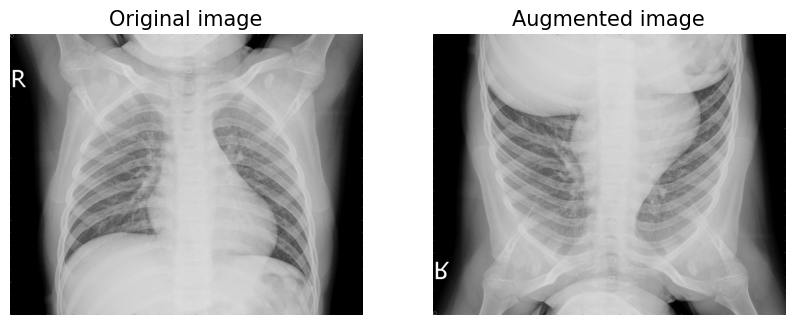
\includegraphics[width=\textwidth]{img/augmented-image-1588951790.png}
    \caption{Flipping an image upside down is not applicable in CAD context}
    \label{fig:upsidedownxray}
  \end{figure}

\subsection{Horizontal flip} \label{subsec:horizontalflip}
This data augmentation is achieved by reversing the pixel values horizontally.
The resulting image would look like a mirror flip from left to right of the same image.

\begin{figure}[H]
    \centering
    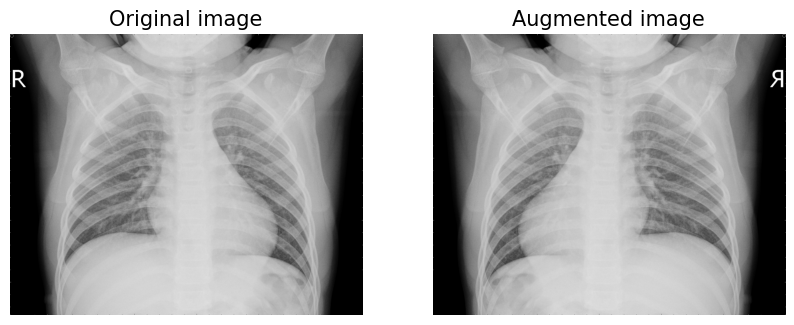
\includegraphics[width=\textwidth]{img/augmented-image-1588951788.png}
    \caption{Horizontal flip augmentation}
    \label{fig:horizontalflipxray}
\end{figure}

\subsection{Random zoom augmentation} \label{subsec:randomzoom}
Also knows as random cropping augmentation.
This argumentation applied by randomly sampling a certain percentage of the original image and either adding padding to a sampled area or rescale the sampled area with interpolation to produce an image of the same shape as the original image.
It is important to choose an appropriate percentage for this argumentation.
The percentage should be chosen in a way that it would not omit the area of interest in the image.
For the purpose of my project, this argumentation must be applied such a way that it would not leave any part of the lungs outside of the image. 
As an example figure \ref{fig:randomzoomxray}, is applied with 10\% of random zoom and it is a considerable level for this dataset.

\begin{figure}[H]
    \centering
    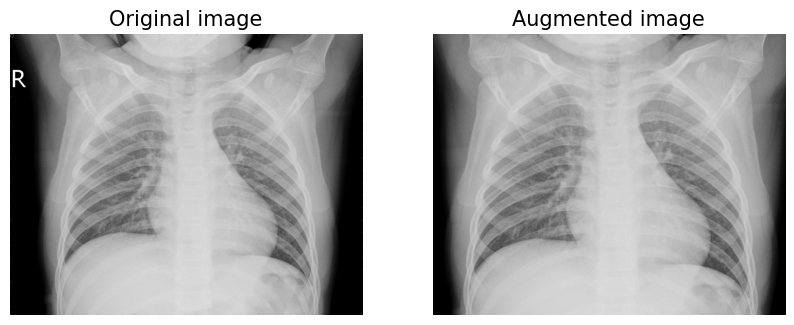
\includegraphics[width=\textwidth]{img/augmented-image-1588951794.png}
    \caption{Random zoom augmentation}
    \label{fig:randomzoomxray}
\end{figure}

\subsection{Changing brightness or saturation} \label{subsec:brightness}
These argumentations either change the brightness or saturation of the image to create an augmented image.
Saturation is done by converting RGB images to HSV (Hue Saturation Value) then multiplying saturation channel with saturation factor chosen for the augmentation.

Brightness augmentation also works a similar way.
RGB values of the image are converted to float representation then applied brightness factor to the values.

\begin{figure}[H]
    \centering
    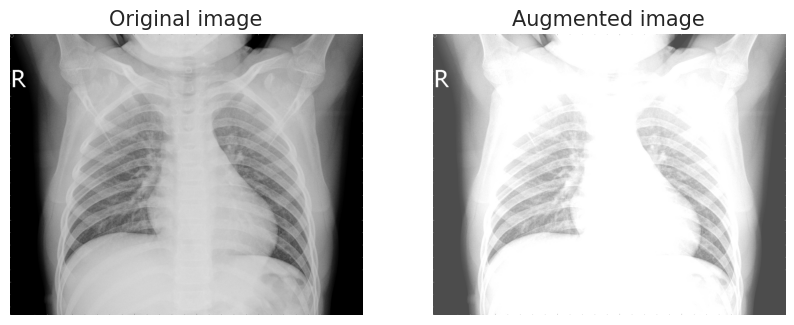
\includegraphics[width=\textwidth]{img/augmented-image-1596666691.png}
    \caption{Brightness augmentation example}
    \label{fig:brightedxray}
\end{figure}


\section{Data Representation} \label{sec:datarepresentation}
Original and augmented images need to be turned into data representations that machine learning algorithms can process.
Normally, colored images represented with pixel values for red, green and blue (RGB) color channels and values for each pixel in any given channel ranges between 0 to 255.
For the traditional machine learning techniques, each data point should be represented in one vector.
Additionally, pixel values for each color channel need to be turned into a vector by flattening each row of pixel values for a particular color channel.
After applying the same step to each channel flattened, channel vectors should be appended one after another to get the final vector for the image.
Given that the model size cannot change during training, each image should be resized to the same shape before representational vector is created (e.g. $\textbf{\textit{x}} = [x_1, x_2, \ldots, x_n]$).

Representation for CNNs, however, require different processing because the convolution operation requires locality of the data points to be taken into consideration.
Therefore the most common approach is to represent each colour channel of the image as an array of vectors which commonly know as \emph{matrix}.
Because the coloured image has three colour channels each matrix for the channels should be combined as a multi-dimension matrix.
This multi-dimensional matrix representation usually referred to as \emph{tensor}.

Much like input data, the label for each image should also be represented in appropriate mathematical entity to be able to process in training.
Because this problem has only two classifications most used method is to encode each class in binary (e.g. 1 for pneumonia and 0 for normal).
However it can also be represented in one-hot encoding, which will return a vector for each label includes binary values for each class (e.g. $[0, 1]$ for pneumonia and $[1, 0]$ for normal).


\section{Limitations of the Dataset} \label{sec:datalimitations}
Although dataset I have chosen is well designed and validated, some aspects of data have undesired properties.
First of such property is the size of the validation data.
As I mentioned earlier dataset has a folder where it hosts validation files.
Within this folder, there are sixteen images where each class have eight images each.
This is significantly small validation dataset and would reduce the bins for each available accuracy step significantly.
For example, making one error in the validation data will result in accuracy declining from 100\% to 93.75\%.

Second undesired property is the high variance of the image resolutions.
Having such a high variance in image resolution makes it difficult to choose the right resolution to resize all the images.
To show the variance within the data I have added a density plot that illustrates the height and width of the images and their distribution in Figure \ref{fig:imagedimensions}.

\begin{figure}[H]
    \centering
    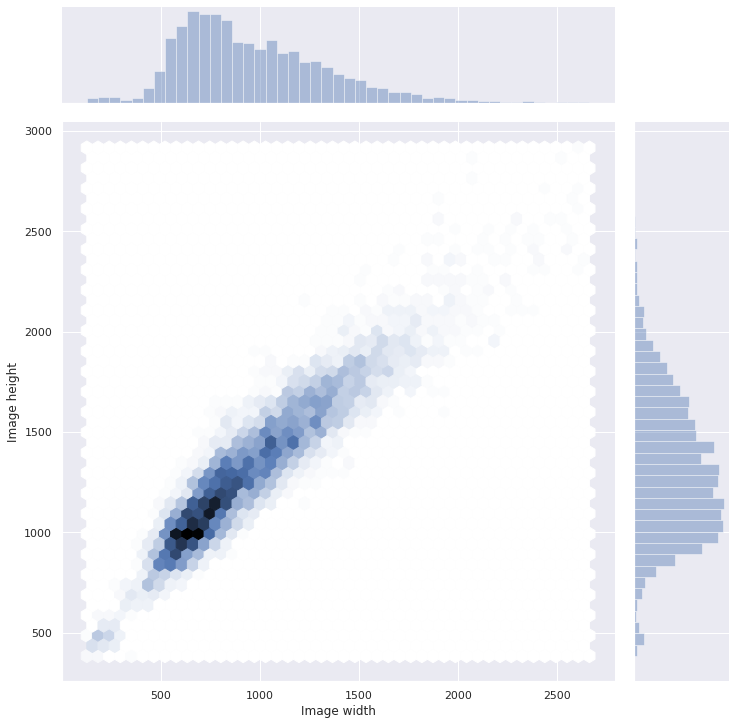
\includegraphics[width=\textwidth]{img/image_dims_density.png}
    \caption{Density plot of image dimensions}
    \label{fig:imagedimensions}
\end{figure}

This graph gives an insight into what resolution for the image should be chosen to have minimal informal loss and distortion in the final image. As we can see most of the images have shape above $500 \times 500$, therefore any resolution below this shape would be an appropriate choice for the training. 

\section{Data Processing} \label{sec:dataprocessing}
Inline with the information provided in section \ref{sec:datarepresentation}, I have designed two separate data processing pipeline.
First pipeline created for data processing for so-called traditional machine learning algorithms such as Random forest or Support vector machine (SVM) that will be used in performance benchmarking.
This pipeline does the flattening of the X-ray images discussed and depends on open-source software libraries keras~\cite{keras} and numpy~\cite{numpy}.

The second pipeline is created for pre-processing of CNN models which would be used in the majority of the time in training and testing.
The module is designed to be lightweight with minimal dependencies. Only third party open source libraries used are, Numpy and the TensorFlow~\cite{tensorflow}.
Although TensorFlow has high-level Keras module that allows easier implementation for data pipeline, I have decided on building data processing pipeline in tf.data module of the TensorFlow library.
Building my pipeline in tf.data meant that I have to build all of the implementations from scratch myself but it also allowed me to build more flexible and more performant pipeline I could have had than the other alternative. 
The goal of having faster training runs and ultimately having shorter prototyping time only achievable if the training is fast enough to feed data into powerful hardware accelerators.
Otherwise, the process will become a bottleneck in the training because the processing unit whether it is GPU or any other device will remain idle until the data fed into the system.
Tf.data designed with parallelization in mind that carries out the process of fetching next data batch while the training for the current batch is in progress so the next batch can be ready as soon as the training is finished.
Providing that all the augmentations and pre-processing will be done in CPU while GPU is training on the previous batch in effect means all the augmentations are computationally free.


At the beginning of this chapter, I point out that the dataset for this project has an imbalance problem.
Building the data pipeline with the tf.data also meant that I am able to eliminate this issue by making a custom pipeline operation that creates a balanced training set.
With the flexibility provided, I was able to apply the augmentations to only minority class of the dataset and add this new training example to training set until I have the same number of examples for both classes.



%%%%%%%%%%%%%%%%%%%%%

% Talk about the decisions for image size and how it relates to information loss and preservation. Briefly mention the high variance of the image sizes and image resizing options and choice.
% Discussing different representation of the dataset will be covered.
\clearpage